\chapter{\ifproject%
    \ifenglish Project Structure and Methodology\else โครงสร้างและขั้นตอนการทำงาน\fi
  \else%
    \ifenglish Project Structure\else โครงสร้างของโครงงาน\fi
  \fi
 }

ในบทนี้ จะกล่าวถึงหลักการ,  การนําทฤษฎีที่เกี่ยวข้องมาประยุกต์ใช้  และการออกแบบของระบบ


\makeatletter

% \renewcommand\section{\@startsection {section}{1}{\z@}%
%                                    {13.5ex \@plus -1ex \@minus -.2ex}%
%                                    {2.3ex \@plus.2ex}%
%                                    {\normalfont\large\bfseries}}

\makeatother
%\vspace{2ex}
% \titleformat{\section}{\normalfont\bfseries}{\thesection}{1em}{}
% \titlespacing*{\section}{0pt}{10ex}{0pt}
\section{โครงสร้างของระบบ}
% \ref{fig:Overall project structure}

% app -> streaming -> ci classify -> results -> Display -> add to cart -> payment -> order
Application โทรศัพท์มือถือ จะสามารถ classify สินค้าได้โดย application จะการถ่ายภาพของสินค้า และทำการ streaming ผ่าน WebSocket
ไปยัง server ที่มี Computational Intelligence ทำหน้าที่ classification ข้อมูลที่ได้รับเข้ามา  และตอบกับข้อมูลชนิดสินค้าและราคา กลับไปยัง application
ผู้ใช้งาน application จะสามารถเพิ่มสินค้าที่ application ถ่าย ไปยังตะกร้าสินค้า และสามารถ กดจ่ายเงินซื้อสินค้าได้

โดยร้านค้าจะการ บันทึกประวัตืการซื้อขาย ของสินค้าภายในร้านทำให้สามารถจัดการ จำนวนของสินค้าภายในร้าน โครงสร้างของระบบ CapSnap จะเป็นดังรูป \ref{fig:Overall project structure}



\begin{figure}[h]
  \begin{center}

    \vspace{0.5cm}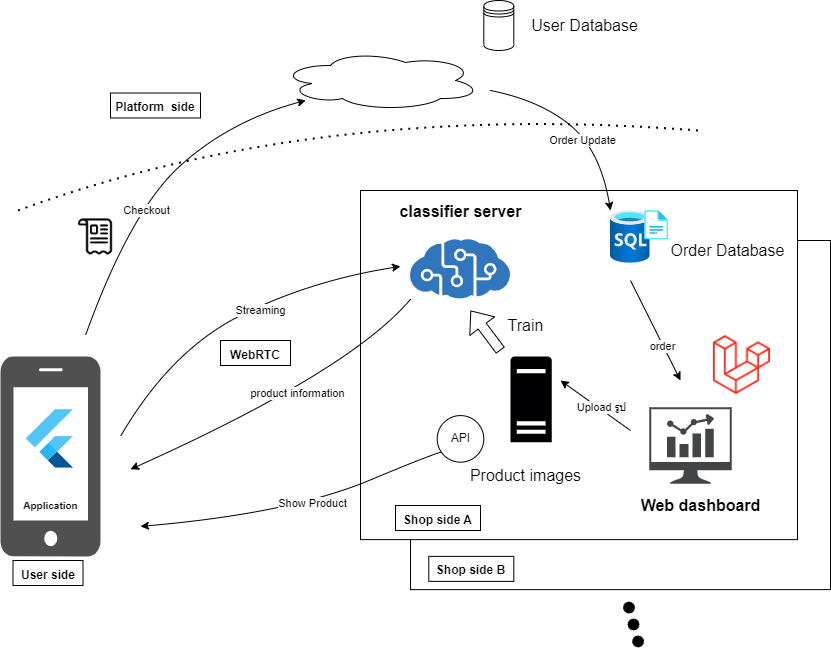
\includegraphics[scale=0.3]{pic/overall_2.png}
  \end{center}

  \caption[Overall project structure]{Overall project structure}
  \label{fig:Overall project structure}
\end{figure}

\newpage
\subsection{แผนภาพกระแสข้อมูล (Data Flow Diagram)}
จากขั้นตอนการทำงานของระบบ  และการ Communication ของ application และ server ของร้านค้า
จะมีโครงสร้างของ Data Flow Diagram ดังรูป \ref{fig:Data Flow Diagram}
\begin{figure}[h]
  \begin{center}

    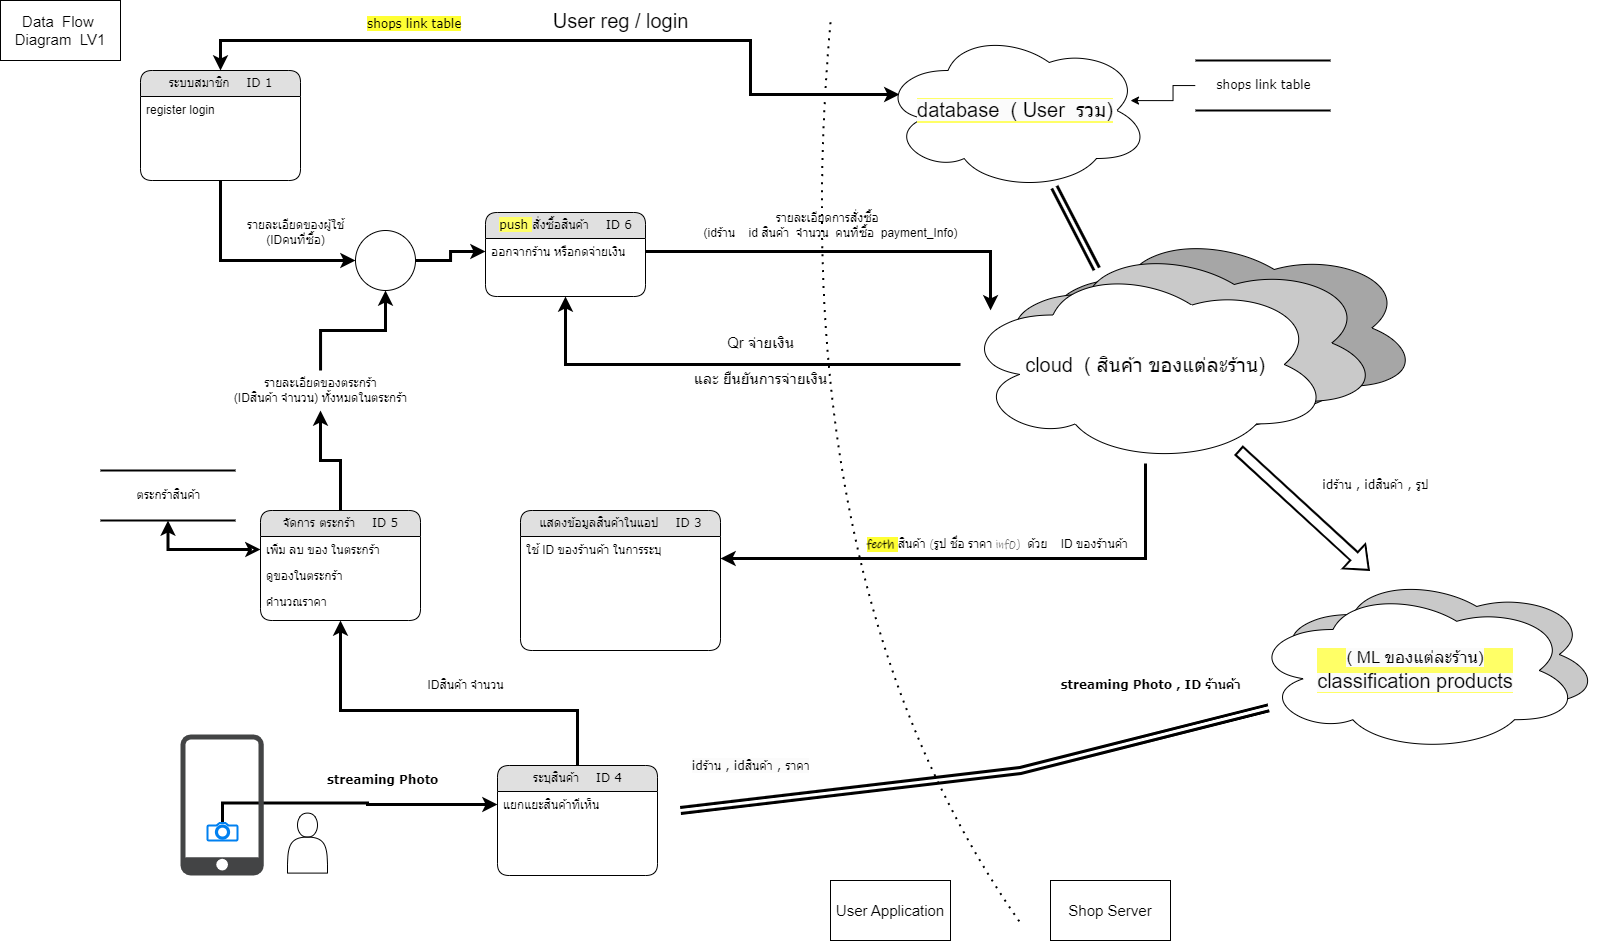
\includegraphics[scale=0.25]{pic/dataflow-lv0.png}
  \end{center}

  \caption[Data Flow Diagram]{Data Flow Diagram}
  \label{fig:Data Flow Diagram}
\end{figure}



\section{เตรียมชุดข้อมูลฝึกสอน}
ข้อมูลที่ใช้ในการ train model ใช้รูปภาพจากสินค้าสินค้าจากห้อง 422  ทำการจัดเก็บข้อมูลรูปภาพ โดยใช้กล้องมือถือ
ในการถ่ายภาพโดยสินค้า 1 class (ชนิด) ทำการถ่ายภาพ 8 รูป ในมุมที่แตกต่างกัน
โดยโมเดลในโครงงานนี้จะใช้สินค้าทั้งหมด 51 class และเพิ่มอีก 1 class สำหรับพื้นหลัง (background class)
รวมเป็น 52 class
จัดเก็บใน Google Drive ดังรูป  \ref{fig:Google Drive} โดยทำการแยก รูปภาพตามหมวดหมู่ และทำการดึงข้อมูลมา train ผ่าน Google Colab
\begin{figure}[h]
  \begin{center}

    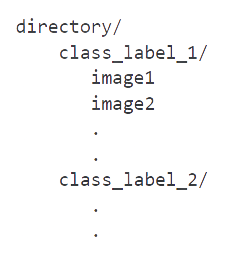
\includegraphics[scale=0.4]{pic/model/st.png}
  \end{center}

  \caption[Google Drive]{Google Drive}
  \label{fig:Google Drive}
\end{figure}
โดยในแต่ละรูป จะเป็นข้อมูล Array ขนาด 224x224x3

\section{K-Fold Cross Validation}

เพื่อตรวจสอบว่า model ที่เราทำการสร้าง ไม่ว่าจะเจอ dataset ที่ข้อมูลแตกต่างกันในแต่ละ fold ก็จะได้ accuracy ที่มีความใกล้เคียงในแต่ละ fold โดยที่ไม่แม่นยำแค่บาง dataset ซึ่งเป็นการ bias ต่อ dataset


\begin{center}
  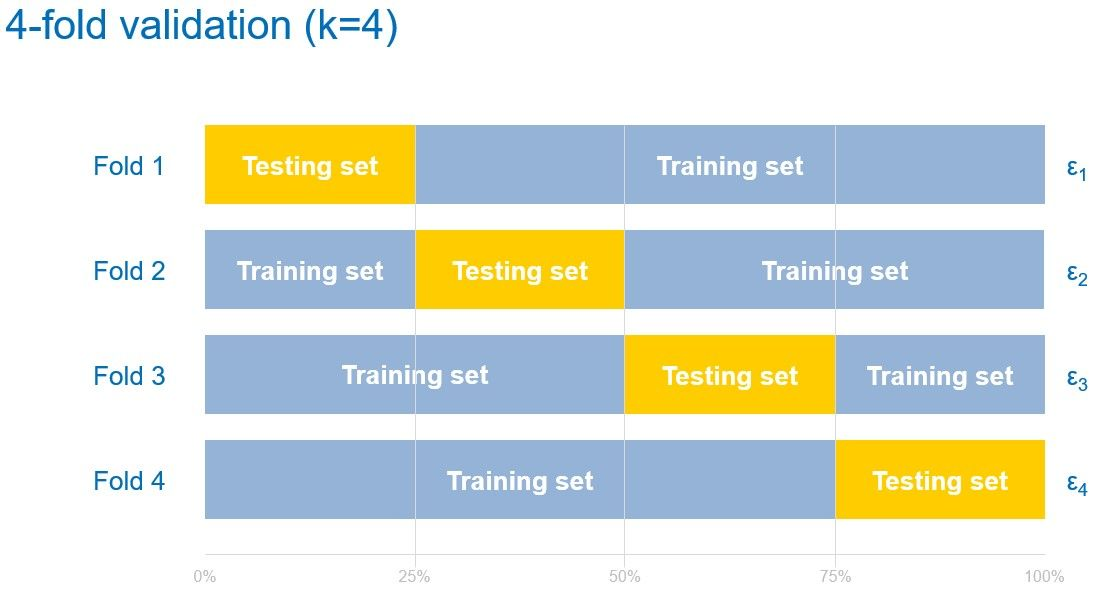
\includegraphics[scale=0.3]{pic/model/CrossValidation.png}\cite{CrossValidation}
\end{center}

ซึ่งในโครงงานนี้ ได้ทำการแบ่ง dataset เป็น ทั้งหมด 4 fold ดังรูป \ref{fig:Dataset}
โดยใน dataset แต่ละ fold ก็จะทำการ augmentation เพื่อเพิ่มจำนวนข้อมูลที่ใช้ในการ train model ของแต่ละ fold
\begin{figure}[h]
  \begin{center}

    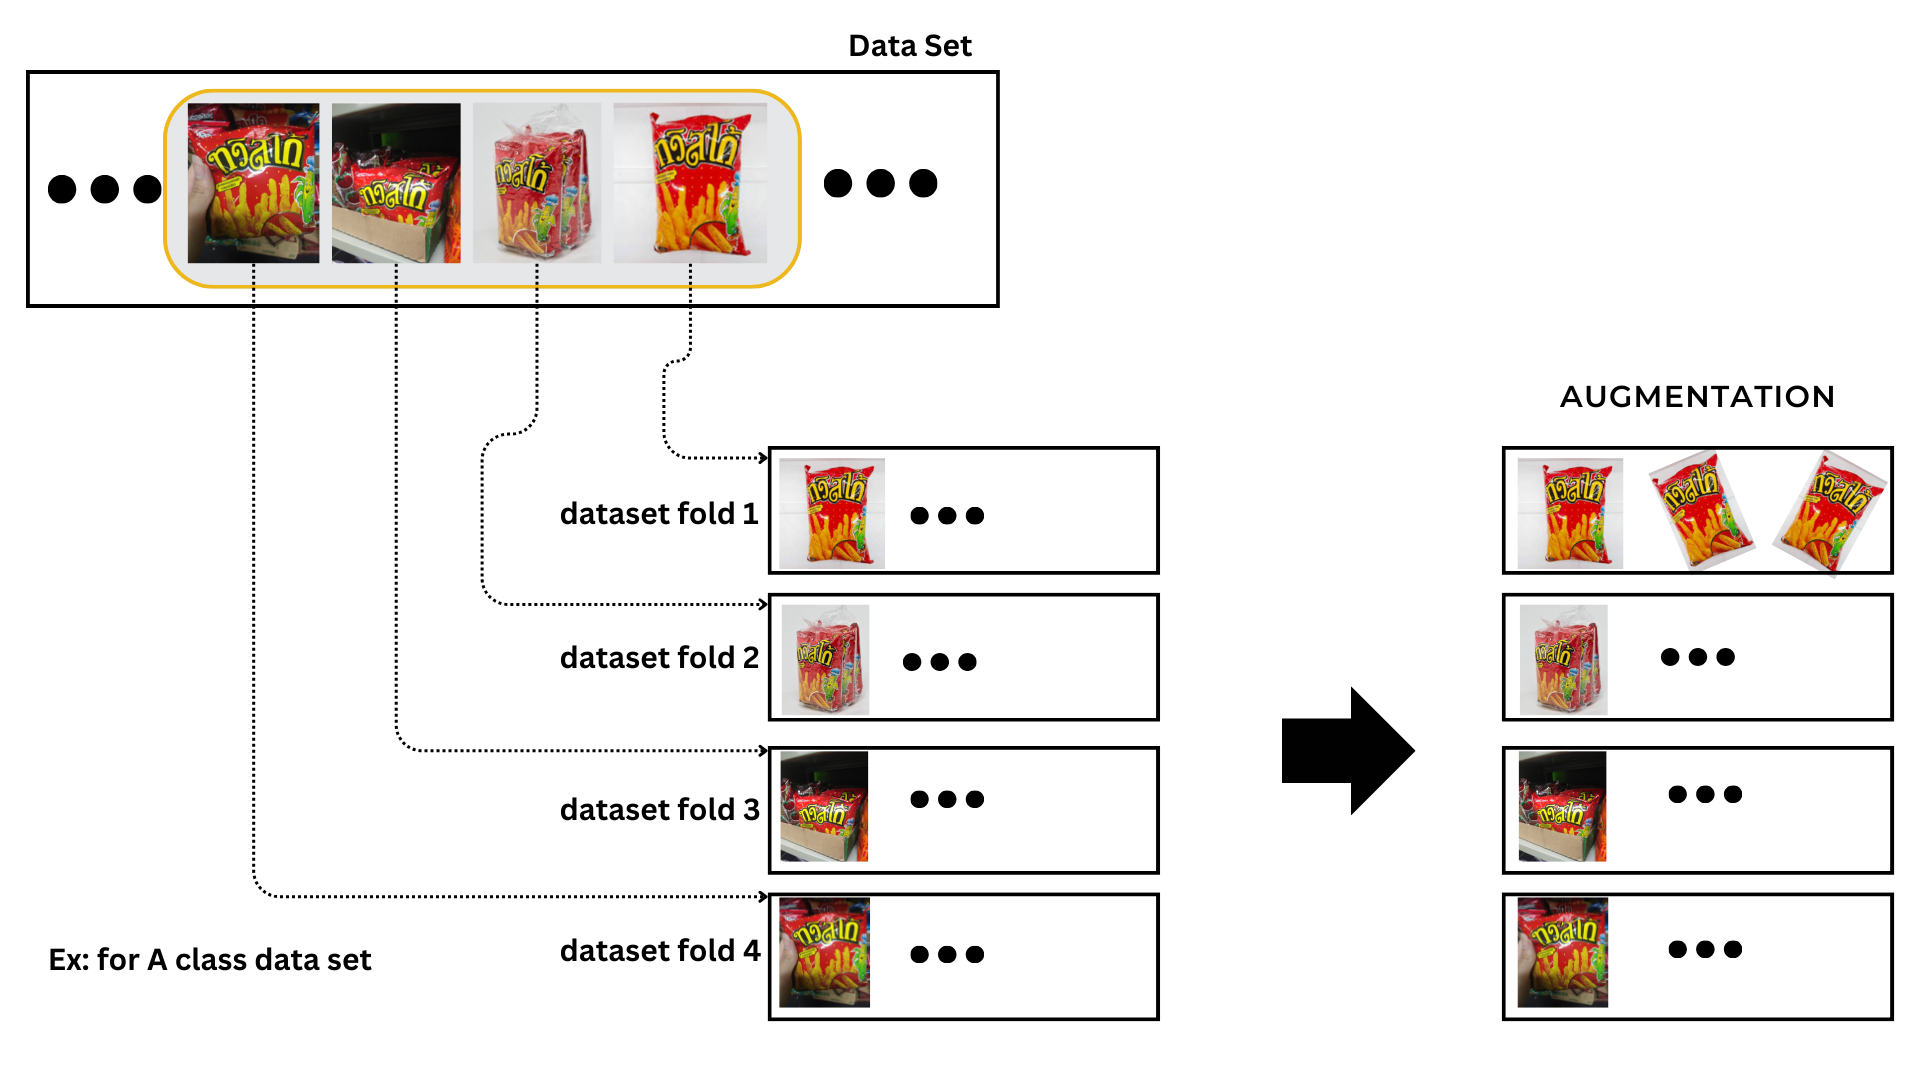
\includegraphics[scale=0.25]{pic/model/fold_aug.png}
  \end{center}

  \caption[Dataset]{Dataset}
  \label{fig:Dataset}
\end{figure}

\newpage



\section{Data augmentation การเพิ่ม traing data}
เพื่อให้มี train dataset ในจำนวนมาก
โดยในแต่ละ 1 รูปภาพที่ถ่าย ซึ่งเป็นรูปภาพ RGB ขนาด 224x224 pixel
นำไปสร้างเป็นรูปภาพใหม่ โดยใช้วิธีการ หมุน และ กลับด้าน ด้วยมุม -20,-15,-10,-5,0,5,10,15,20 องศา
โดย 1 รูปภาพผ่านการ generate datasets จะกลายเป็น 18 รูปภาพซึ่งมีความแตกต่างกันเล็กน้อย ตามรูป \ref{fig:Dataset generator}

\begin{figure}[h]
  \begin{center}

    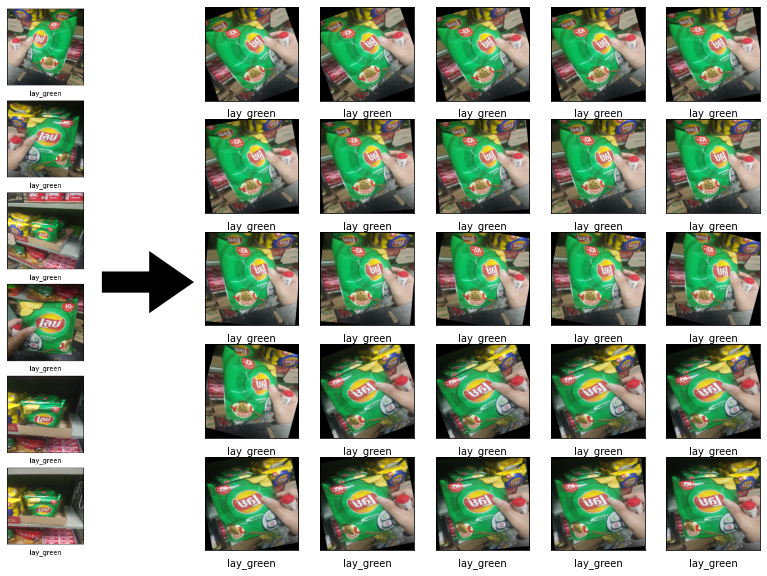
\includegraphics[scale=0.4]{pic/model/lay_genmore.png}
  \end{center}

  \caption[Dataset generator]{Dataset generator}
  \label{fig:Dataset generator}
\end{figure}




\newpage
\subsection{Model Architecture}
โดยโมเดลในโครงงานนี้จะใช้ Xception pre-trained ซึ่งเป็น Convolutional Neural Network ซึ่งมีความลึก 71 layers.
เป็นโมเดลที่ผ่านการจากรูปภาพต่าง ๆ มากกว่าล้านรูปภาพจาก ImageNet database .
ซึ่งจะมีโครงสร้างดังรูป


\begin{center}
  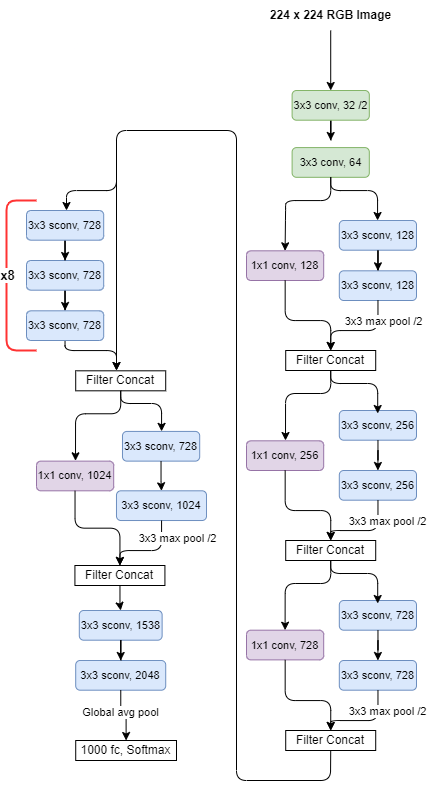
\includegraphics[scale=0.35]{pic/model/x_1.png}\cite{Xception}
\end{center}


โดยการนำ Xception model มาใช้ในการแยกคุณลักษณะเด่นของรูปภาพ  และ สร้างโมเดลมาต่อท้ายเพื่อ
เรียนรู้ลักษณะเด่นจากที่ Xception ทำการแยกออกมาได้


% transfer learning - Xceptionโดย pre-train 'Xception' model 



\begin{center}
  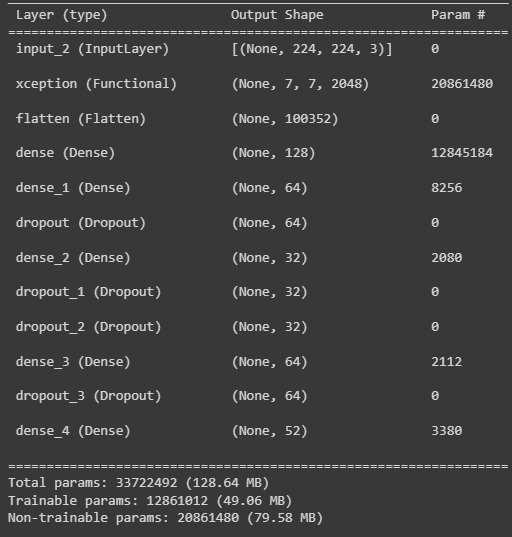
\includegraphics[scale=0.5]{pic/model/model.png}
\end{center}

ซึ่ง model ที่จะใช้ก็จะเป็น Xception model ที่รับ Input ขนาด 224 x 224 x 3 ตามขนาดรูปภาพ 224x224 pixel และตาม layer RGB

โดย Xception เป็น model ตั้งต้นที่่ผ่าน pre train model จะทำหน้าที่เป็น feature exercitation ลักษณะเด่นของรูปภาพ
โดย Xception จะถูก lock ค่าของ weight เอาไว้เพื่อไม่ไห้ค่าของ weight ที่ได้เรียนรู้ข้อมูลมาจาก ImageNet หายไป
ซึ่ง exercitation มี weight ทั้งหมด 20 ล้าน parameter

และนำ layer มาต่อท้าย model ด้วย fully connected node ที่เรียกว่า Dense layer จำนวน 32 node และ 16 node และ
layer สุดท้าย ซึ่งมีขนาดเท่ากับจำนวน class ของสินค้า ซึ่งทำหน้าที่เป็น classifier
โดย Dense layer ซึ่งเชื่อมกันแบบ fully connected ที่สามารถ เรียนรู้และปรับค่าของ weight ได้
ในโครงสร้างทดสอบนี้จะมี weight ที่่สามารถเรียนรู้ หรือ เปลี่ยนแปลงได้ 12 ล้าน paramiter


\section{classification products}
จากรูปภาพใน 52 class ผ่านการ generate datasets จะมี dataset ทั้งหมด 4432 sample
ทำการแบ่งเป็น train 3546 sample และ  886 sample สำหรับการ evaluate
โดยจาก train 3546 แบ่ง 50\% สำหรับการ validation ในระหว่างการ train model

สำหรับเป็น service ในการ classify products ของ application ผ่าน aiortc  และเว็บ WebSocket



\newpage

\section{การพัฒนา Mobile Application}
ใช้ Flutter ในการสร้าง Mobile Application ในส่วนของผู้ใช้โดยใช้ service ของ WebSocket ติดต่อกับ Classification server ที่ได้ทำการฝึกสอนไว้แล้ว
โดยจะแอพลิเคชันจะมีฟังก์ชันที่ทำการสตรีมมิ่งภาพสินค้าที่ลูกค้าถ่ายผ่าน WebSocket ไปยัง server ของทางร้านซึ่งมี Model classifier อยู่
จากนั้น Server ของทางร้านจะ Classifiy ว่าเป็นสินค้าชนิดใด และตอบกลับมายังแอพลิเคชันเพื่อแสดงผลให้กับผู้ใช้งาน
\subsection{Requirement Specification}

\begin{enumerate}
  \item ผู้คนทั่วไปสามารถลงทะเบียนเข้าใช้งานได้ผ่าน SSO อีเมล์ และหมายเลขโทรศัพท์มือถือ
  \item สามารถเชื่อมต่อกับข้อมูลร้านค้าได้ผ่านการแสกนคิวอาร์โค้ดเข้าใช้งานร้านค้า
  \item สามารถใช้กล้องโทรศัพท์มือถือแสกนสินค้าเพื่อสตรีมภาพ Classification server เพื่อทำการดึงข้อมูลสินค้าจาก Server ของร้านค้ามาแสดงผลบนแอพลิเคชัน
  \item สามารถเพิ่มหรือลดสินค้าในตะกร้าได้
  \item สามารถทำการชำระเงินได้ผ่าน Payment gateway ในตัวแอพลิเคชัน
  \item สามารถ Checkout จากร้านค้าผ่านการแสกนคิวอาร์โค้ดออกจากร้านค้า

\end{enumerate}


\section{การเตรียมฐานข้อมูล}
ในการเก็บฐานข้อมูลจะแบ่งเป็นฐานข้อมูลสองตัว โดยใช้ Supabase
ในการสร้างโครงการ และจัดฐานข้อมูลทั้งหมดแบบ SQL  โดยจะเป็น ฐานข้อมูลของระบบ และ ฐานข้อมูลในแต่ละร้านค้า




\subsection{ฐานข้อมูลของระบบ}
สำหรับเก็บข้อมูลร้านค้าที่เข้าร่วม และประวัติการซื้อสินค้าของผู้ใช้งานแอพลิเคชันมือถือ ซึ่งมี Database schema ดังนี้
\begin{figure}[h]
  \begin{center}

    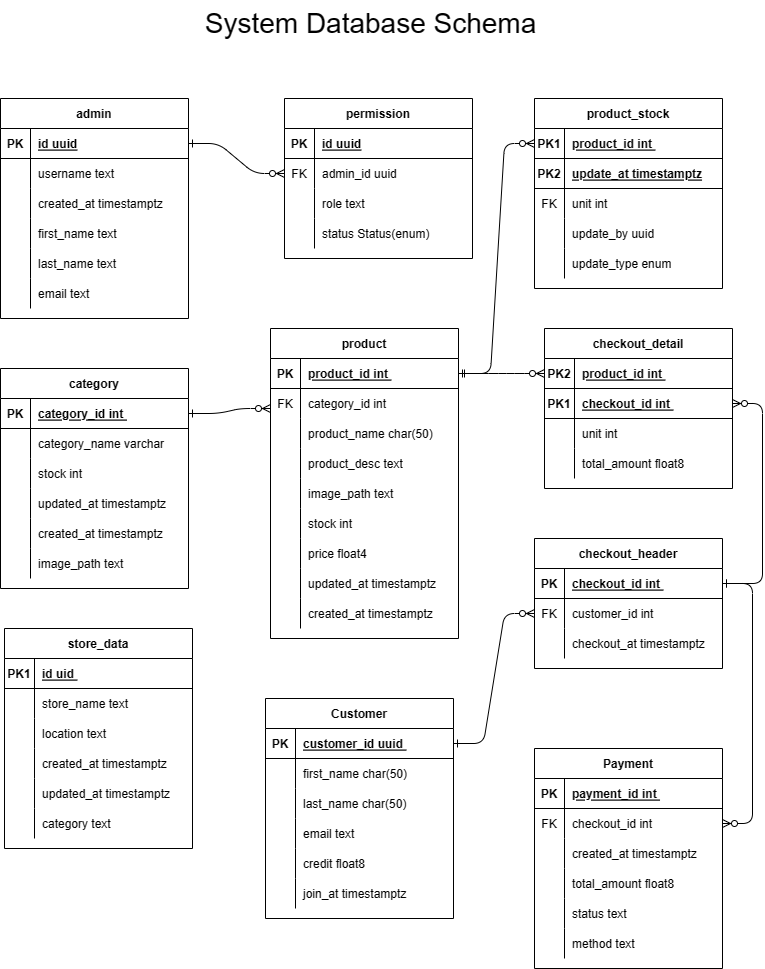
\includegraphics[scale=0.3]{pic/database.png}
  \end{center}

  \caption[System Database Schema]{System Database Schema}
  \label{fig:Mobile Application Database Schema}
\end{figure}
แสดงแผนผังโครงสร้างของดังรูปที่ \ref{fig:Mobile Application Database Schema} ซึ่งออกแบบให้มีฐานข้อมูลทั้งหมด 10 ตาราง ได้แก่ 

\begin{enumerate}
  \item Admin: เก็บข้อมูลของแอดมิน ซึ่งเป็นผู้ที่สามารถเข้าถึงและแก้ไขข้อมูลร้านค้าได้ โดยในร้านหนึ่ง ๆสามารถมีแอดมินได้มากกว่าหนึ่งคน ซึ่งจะเก็บข้อมูลชื่อจริง รหัสผ่าน ที่อยู่อีเมล์ และรูปภาพของแอดมิน โดยมี Primary key เป็นชื่อผู้ใช้ หรือ username
  \item Permission: เก็บสถานะของแอดมิน ได้แก่ Administers และ Super Administers
  \item Product: เก็บข้อมูลขอฃสินค้าแต่ละชนิดได้แก่ ชื่อสินค้า รูปสินค้า จำนวนสินค้าในคลัง ราคาสินค้า คำอธิบายสินค้า และหมวดหมู่สินค้าซึ่งเป็น Foreign key จากตาราง Category และมี Primary key คือ รหัสหรือ product\_id 
  \item Category: เก็บข้อมูลของหมวดหมู่สินค้า ซึ่งประกอบไปด้วยชื่อ และคำอธิบายของหมวดหมู่สินค้า โดยมี Primary key คือ รหัสหมวดหมู่สินค้า หรือ category\_id 
  \item Checkout header: เก็บข้อมูลคำสั่งซื้อสินค้าทั้งหมดของร้านค้า ซึ่งประกอบไปด้วยวันที่ และเวลาที่สั่งซื้อ ยอดขายจากคำสั่งซื้อ หมายเลขระบุตัวตนลูกค้าหรือ customer\_id จากตาราง Customer และรหัสชำระเงิน หรือ payment\_id  จากตาราง Payment ซึ่งมี Primary key คือ หมายเลขระบุคำสั่งซื้อ หรือ order\_id
  \item Checkout detail: เก็บข้อมูลสินค้าที่ถูกซื้อของแต่ละคำสั่งซื้อ โดยเก็บ Foreign key เป็นหมายเลขระบุคำสั่งซื้อ หรือ order\_id จากตาราง OrderHeaders และรหัสสินค้า หรือ product\_id จากตาราง Product ควบคู่กันเป็น Primary key และเก็บข้อมูลอื่น ๆ ได้แก่ จำนวนสินค้าที่สั่งซื้อ และจำนวนเงินที่จ่ายทั้งหมด
  \item Customer: เก็บข้อมูลลูกค้าของร้านค้า โดยเก็บชื่อ username ของลูกค้า และมี Primary key คือ หมายเลขระบุตัวตนลูกค้าหรือ customer\_id 
  \item Product stock: เก็บข้อมูลการเปลี่ยนแปลงจำนวนสินค้าในคลัง โดยเก็บ Foreign key เป็นหมายเลขระบุสินค้า หรือ product\_id จากตาราง Product และจำนวนสินค้าที่เพิ่ม หรือลด มี Primary key คือ ชื่อผู้ใช้งานแอดมินผู้เปลี่ยนจำนวนสินค้าในคลัง หรือ username จากตาราง Admin ควบคู่กับวันที่และเวลาที่ทำการเปลี่ยน หรือ timestamp
  \item Payment: เก็บข้อมูลการชำระเงิน ซึ่งประกอบไปด้วยประเภทการชำระเงิน วันที่ และเวลาของการชำระเงิน และสถานะการชำระเงิน และเก็บ Foreign key เป็นหมายเลขระบุตัวตนลูกค้า หรือ customer\_id  มี Primary key คือ รหัสชำระเงิน หรือ payment\_id 
  \item Store data: เก็บข้อมูลของร้านค้า ได้แก่ ชื่อ สถานที่ัตั้งและ ประเภทร้านค้า
 
\end{enumerate}


\section{การพัฒนา Website Dashboard }


ออกแบบ UI/UX ของ Wedsite Dashboard และ Mobile Application ด้วย Figma
หลังจากการออกแบบ และจัดการตั้งค่าฐานข้อมูลเสร็จแล้ว
ก็จะพัฒนาในส่วนของเว็บไซต์ทางฝั่งร้านค้าโดยใช้ Supabase ในการโฮสติ้งเว็บไซต์
และเชื่อมต่อกับฐานข้อมูลที่ได้ตั้งค่าไว้ โดยใช้ Flask framework
ในการจัดการ API และ Python ในการจัดการระบบ Backend ของเว็บไซต์โดยใช้ SQLAlchemy
ในการดึงข้อมูลจากฐานข้อมูล Requirement Specification ดังนี้

\begin{enumerate}
  \item สามารถเข้าใช้งานได้ผ่านการยืนยันตัวตนเป็น Administers เท่านั้น โดยสามารถมีได้ 1-5 คน
  \item สามารถดูคลังสินค้า และแก้ไขข้อมูลสินค้าในแต่ละชนิดได้แบบเรียลไทม์
  \item สามารถดูสถิติยอดขายสินค้าได้ทั้งแบบรายวัน รายเดือน และรายปี โดยแบ่งได้ 2 แบบ คือตามชนิดสินค้า และประเภทสินค้า
  \item สามารถดูประวัติการขายตามออเดอร์ของลูกค้าแต่ละคนได้ และดูข้อมูลของแต่ละออร์เดอร์ได้
\end{enumerate}

\newpage
 % \begin{center}
 {
  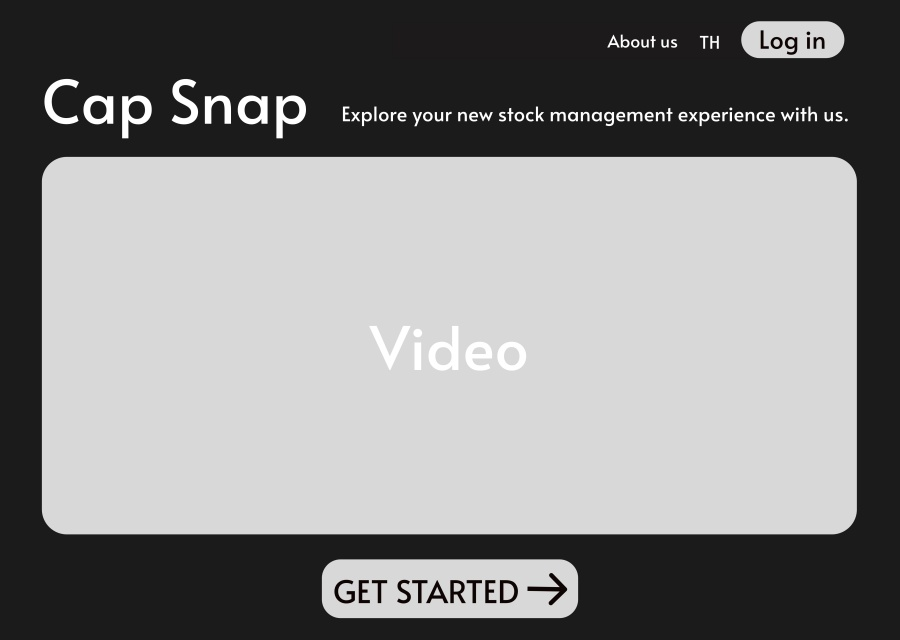
\includegraphics[scale=0.9]{pic/ui/1.jpg}
  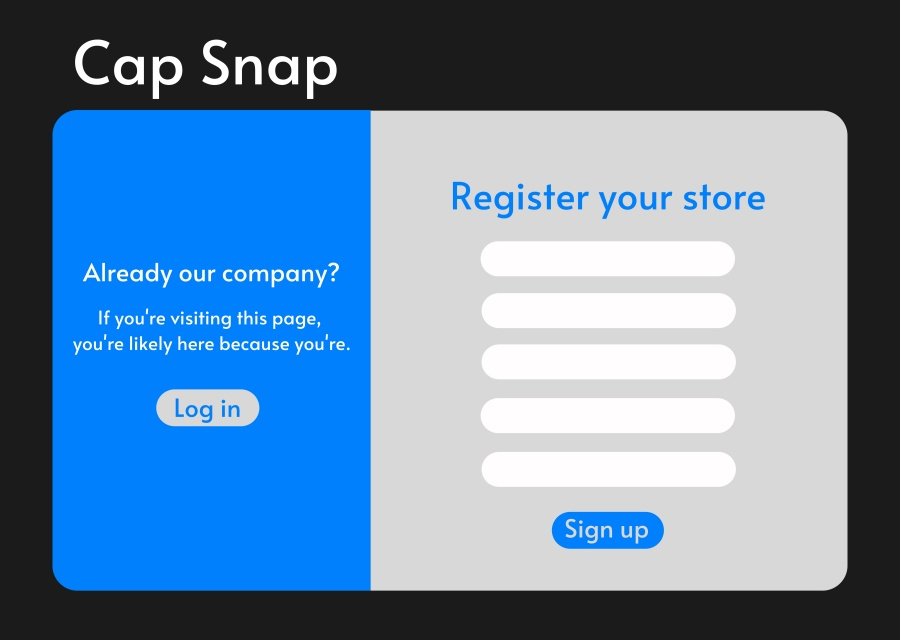
\includegraphics[scale=0.9]{pic/ui/2.jpg}
 }\\
{
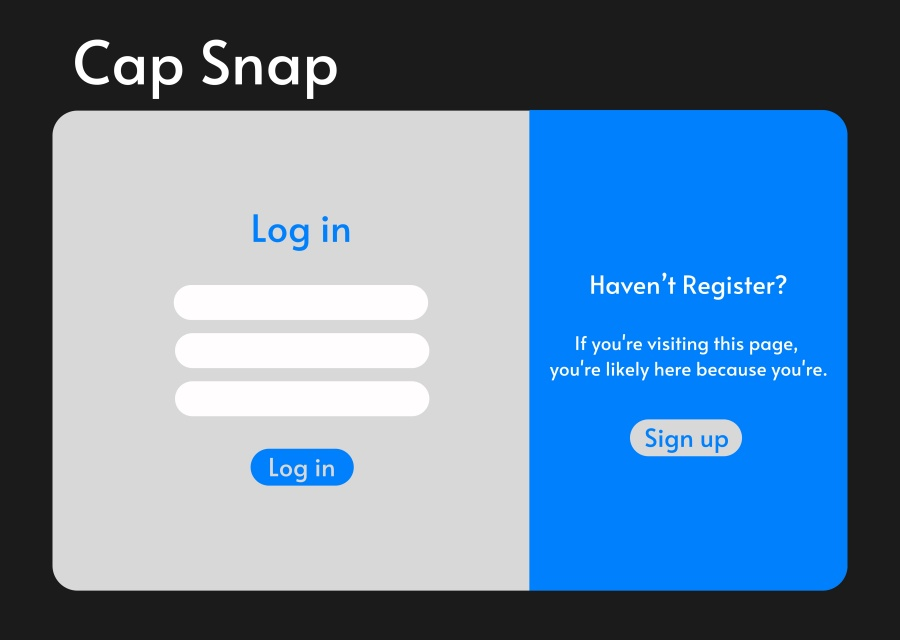
\includegraphics[scale=0.9]{pic/ui/3.jpg}
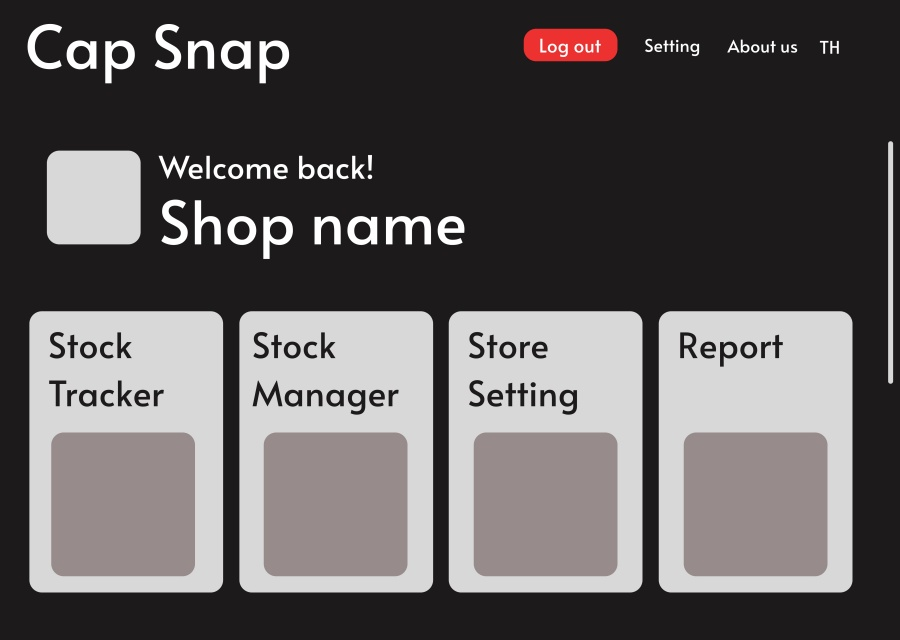
\includegraphics[scale=0.9]{pic/ui/4.jpg}
}\\
{
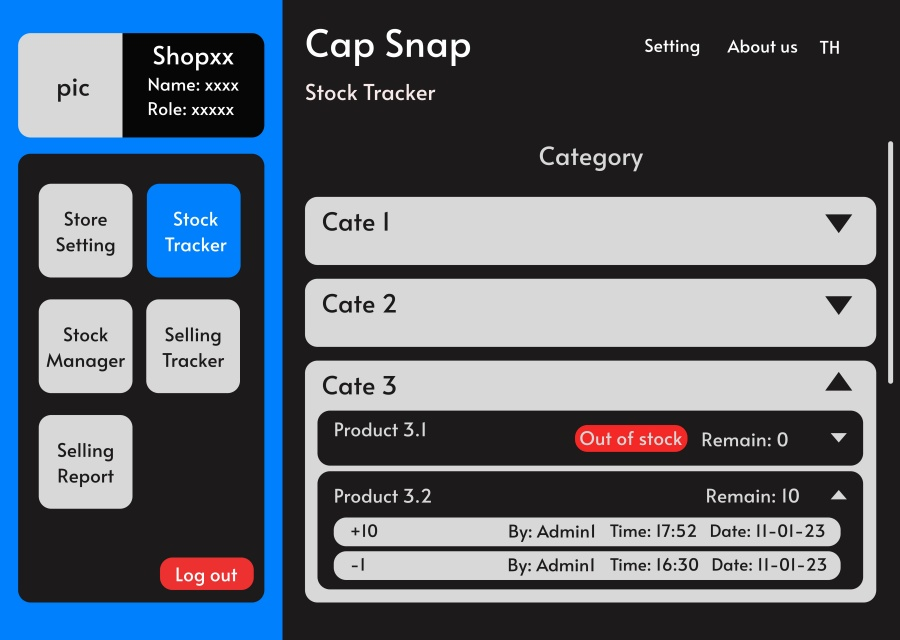
\includegraphics[scale=0.9]{pic/ui/5.jpg}
% 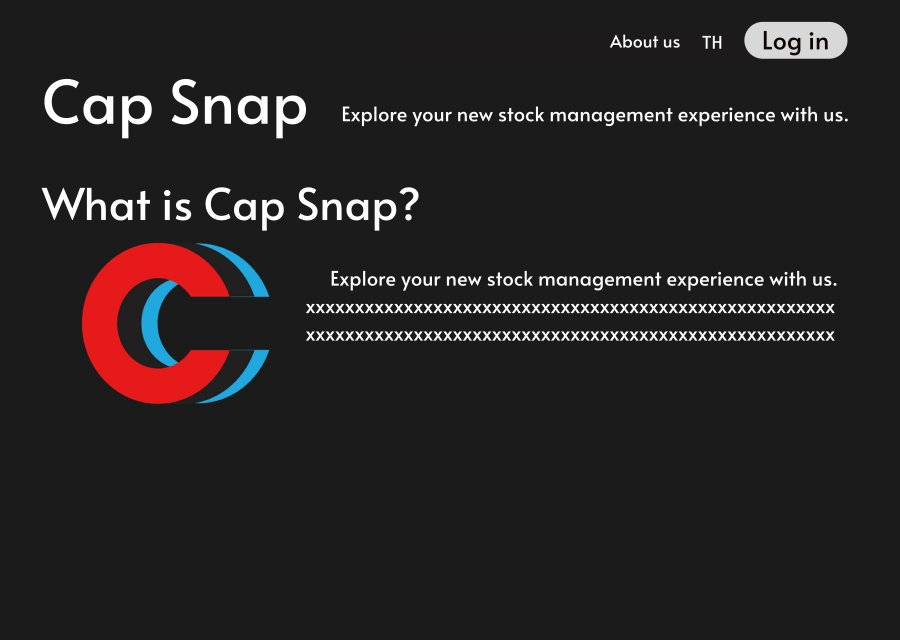
\includegraphics[scale=0.9]{pic/ui/6.jpg}
}\\
{
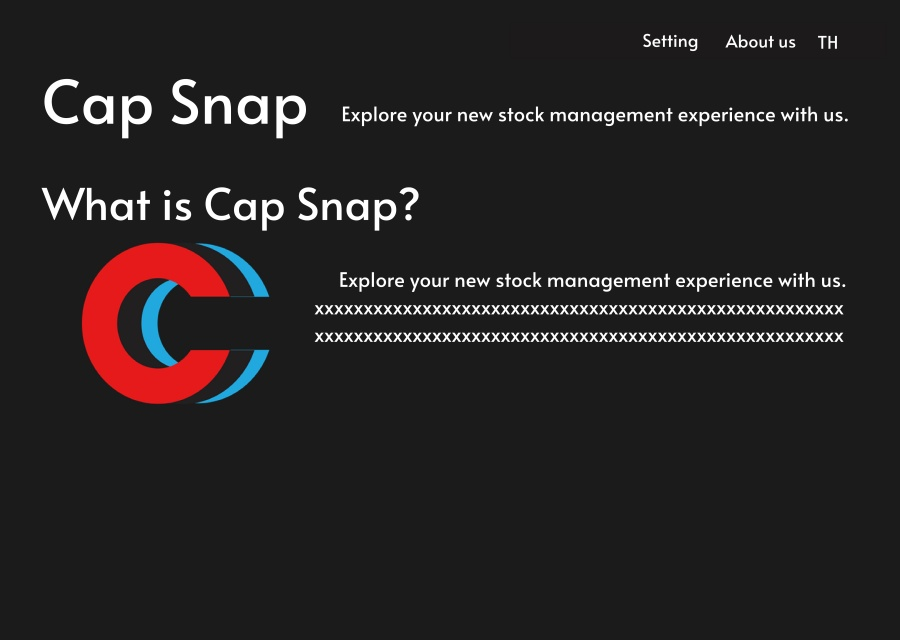
\includegraphics[scale=0.9]{pic/ui/7.jpg}
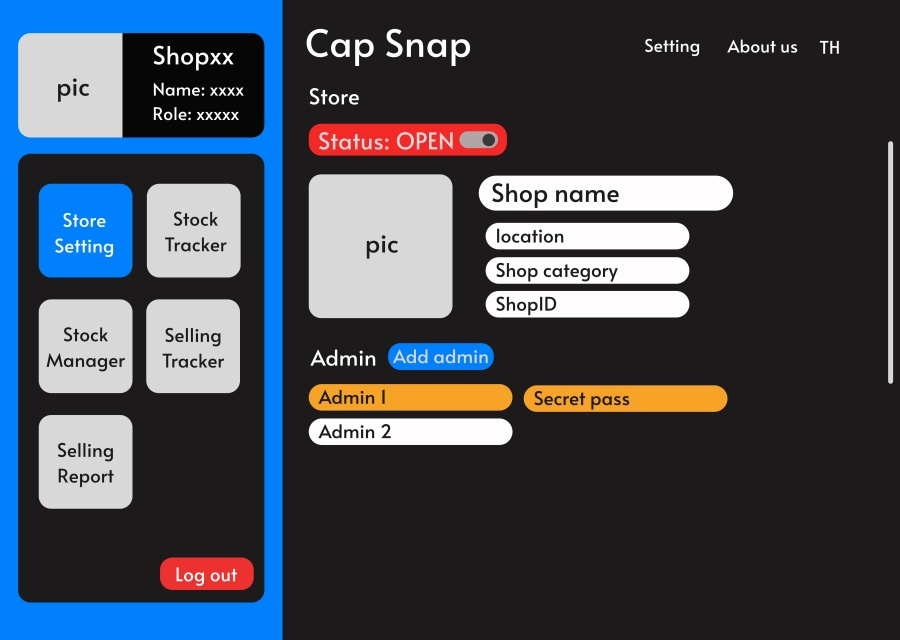
\includegraphics[scale=0.9]{pic/ui/8.jpg}
}\\
{
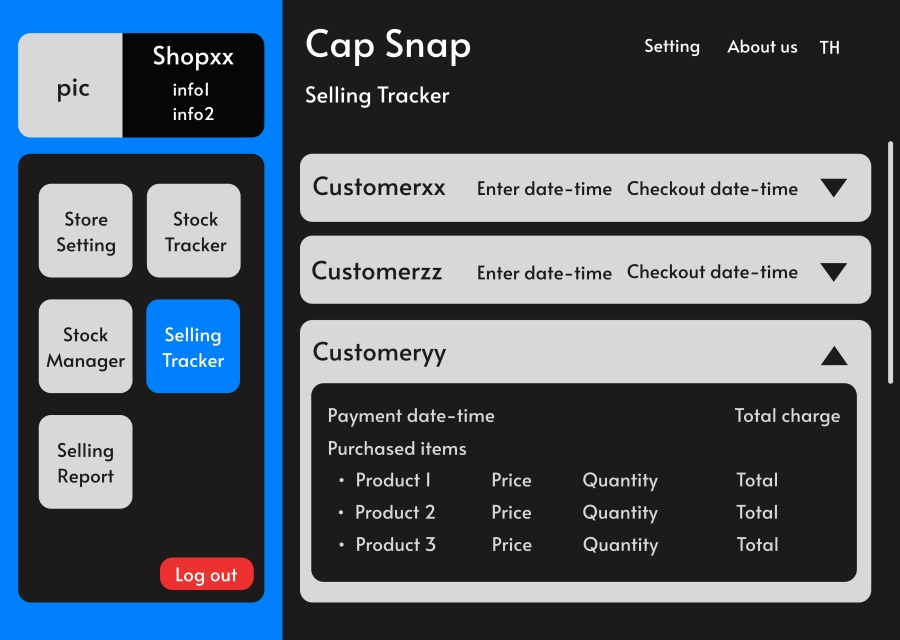
\includegraphics[scale=0.9]{pic/ui/9.jpg}
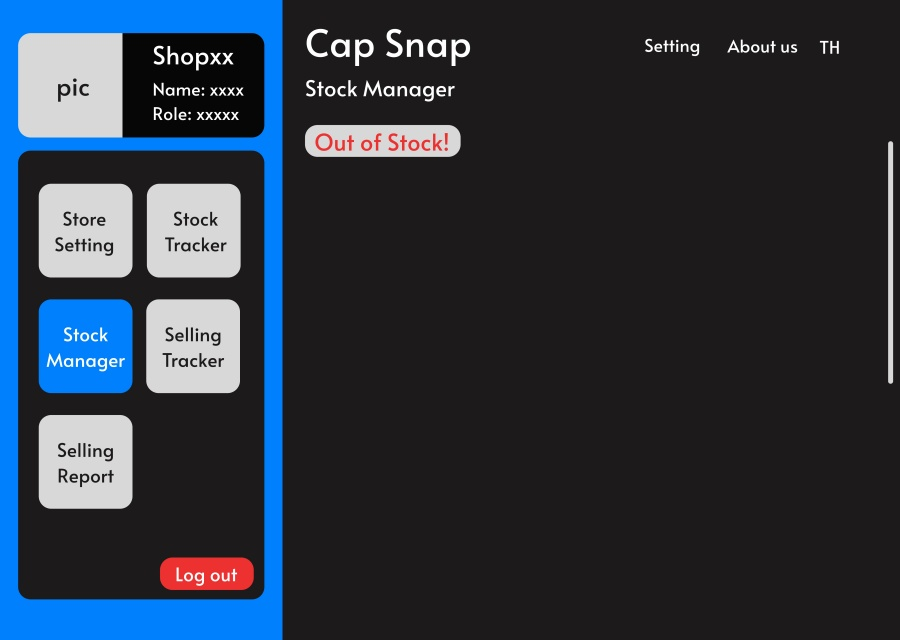
\includegraphics[scale=0.9]{pic/ui/10.jpg}
}\\
{
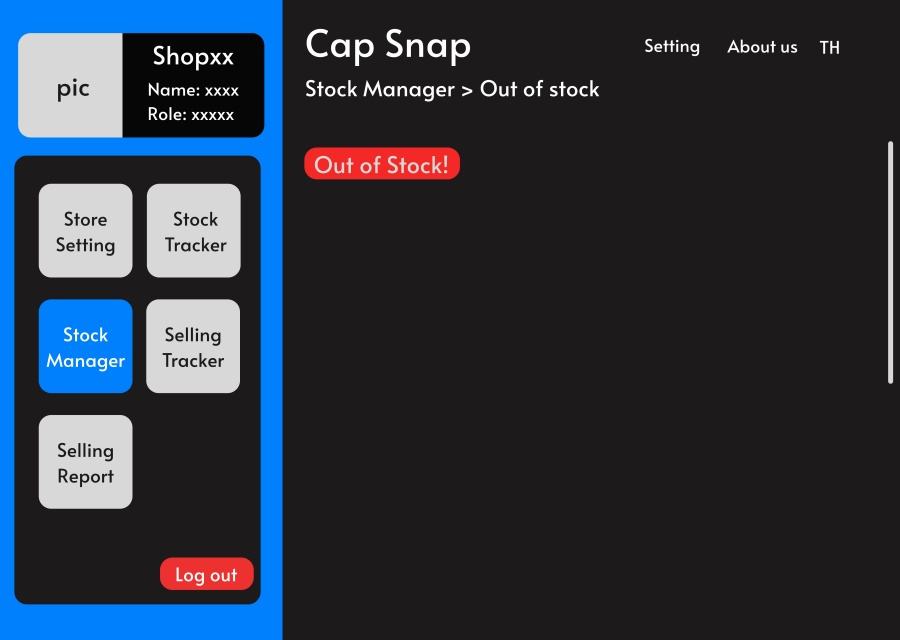
\includegraphics[scale=0.9]{pic/ui/11.jpg}
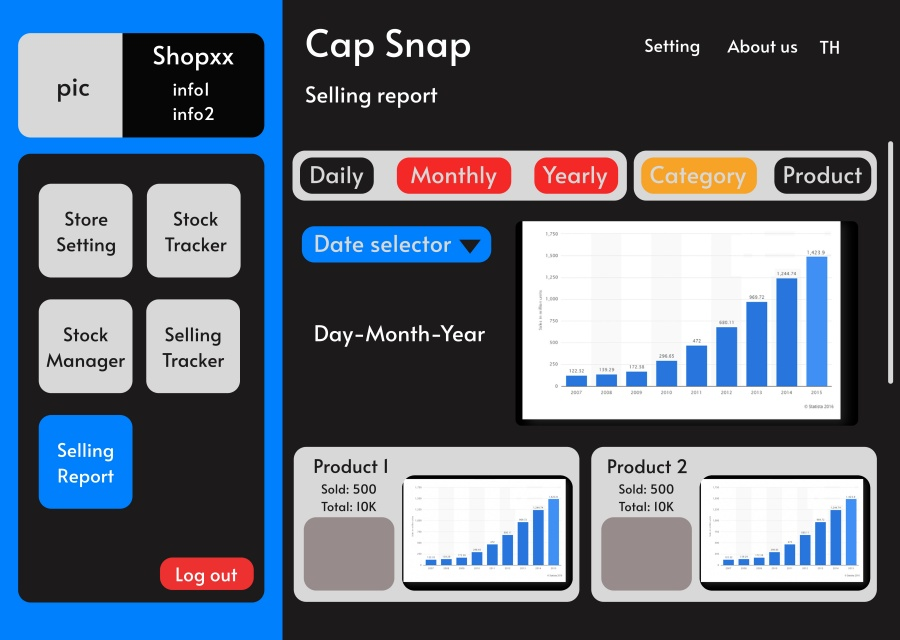
\includegraphics[scale=0.9]{pic/ui/12.jpg}
}


ในส่วนของการออกแบบส่วนสื่อประสานกับผู้ใช้ (GUI) ของ Website Dashboard นั้น ได้กำหนดให้มีหน้าการใช้งานหลักทั้งหมด 11 หน้า ได้แก่
\begin{enumerate}
    \item Get started page: หน้าการเข้าสู่ระบบ หรือลงทะเบียนเข้าใช้งาน
    \item Login page: หน้าการเข้าสู่ระบบ
    \item Register page: หน้าการลงทะเบียนเข้าใช้งาน
    \item Home page:  หน้าแสดงเมนูของฟังก์ชันต่าง ๆ
    \item Store setting page: หน้าการตั้งค่าข้อมูลร้านค้า
    \item Stock tracker page: หน้าการติดตามคลังสินค้า
    \item Stock manager page: หน้าการจัดการคลังสินค้า
    \item Stock manager page > Out of stock page: หน้าการจัดการสินค้าที่ไม่เหลือในคลัง
    \item Selling tracker page: หน้าการติดตามยอดขายตามลำดับคำสั่งซื้อ
    \item Selling report page: หน้าการแสดงผลข้อมูลยอดขายตามรายวัน รายเดือน และรายปี โดยสามารถดูตามหมวดหมู่ของสินค้า หรือแยกตามสินค้าหนึ่ง ๆได้
\end{enumerate}






\section{การทดสอบการทำงานของซอร์ฟแวร์}
การทดสอบการทำงานของระบบ สามารถแบ่งเป็นขั้นตอนดังนี้
\subsection{Unit testing}
การทดสอบความถูกต้องของการทำงานในแต่ละฟังก์ชันหลักของระบบแยกกัน โดยยังไม่รวมแต่ละ Component เข้าด้วยกัน ซึ่งได้แก่
\begin{enumerate}
  \item Classification system
  \item Website dashboard
  \item Mobile Application
\end{enumerate}

\subsection{Integration testing}
การทดสอบการทำงานเมื่อรวมระบบย่อยทั้งหมดเข้าด้วยกัน โดยหลัก ๆ
จะทดสอบในเรื่อง API ว่ามีการรับส่งข้อมูลดุถูกต้องหรือไม่ และทำงานโดยรวมได้ถูกต้องทั้งหมดหรือไม่
\subsection{System testing}
การทดสอบระบบซึ่งแต่ละโมดูลข้างต้นจะถูกรวม และทดสอบเป็นกลุ่ม
เพื่อประเมินความสอดคล้องของระบบว่าทำงานได้ตามที่กำหนดไว้หรือไม่
\subsection{Acceptance testing}
การทดสอบระบบโดยดูภาพรวมของการทำงาน ว่ามีการตอบสนองความต้องการของผู้ใช้ทั้งในส่วนของฟังก์ชันการทำงาน
และประสิทธิภาพการทำงาน ว่าสอดคล้องกับลักษณะของความต้องการของซอฟต์แวร์หรือไม่
โดยใช้การทดสอบแบบ Functional testing (Black box testing)



% \subsection{The Black Kitten}
% One thing was certain, that the WHITE kitten had had nothing to
% do with it:---it was the black kitten's fault entirely



% ~\cite{aiw}. 




%  For the
% white kitten had been having its face washed by the old cat for
% the last quarter of an hour (and bearing it pretty well,
% considering); so you see that it COULDN'T have had any hand in
% the mischief.

%   The way Dinah washed her children's faces was this:  first she
% held the poor thing down by its ear with one paw, and then with
% the other paw she rubbed its face all over, the wrong way,
% beginning at the nose:  and just now, as I said, she was hard at
% work on the white kitten, which was lying quite still and trying
% to purr---no doubt feeling that it was all meant for its good.

%   But the black kitten had been finished with earlier in the
% afternoon, and so, while Alice was sitting curled up in a corner
% of the great arm-chair, half talking to herself and half asleep,
% the kitten had been having a grand game of romps with the ball of
% worsted Alice had been trying to wind up, and had been rolling it
% up and down till it had all come undone again; and there it was,
% spread over the hearth-rug, all knots and tangles, with the
% kitten running after its own tail in the middle.

% \subsection{The Reproach}

